\documentclass[11pt]{beamer}
\usepackage[spanish]{babel}
\usepackage{amsmath} % Mates
\usepackage{graphicx} % Imágenes
\usepackage{subfigure} % subimágenes
\usepackage{ragged2e} % Justificar texto
\usepackage{lipsum} % Texto aleatorio
\usepackage{comment} % Comentar por bloques
\usepackage{xcolor} % Color para las letras
\usepackage{tikz}
\PassOptionsToPackage{demo}{graphicx}
\usepackage[font=scriptsize,labelfont=bf]{caption}


%%%%%%%%%%%%%%%%% Aspecto %%%%%%%%%%%%%%%%%%%
\usetheme{Madrid}
\useinnertheme{circles}
\newenvironment{cirenv}{\only{\setbeamercolor{local structure}{fg=black}}}{} % circulos en las viñetas
%----------------------------------
%\useinnertheme{rectangles}
%\setbeamertemplate{blocks}[default]

%% Para tener bloques sin redondes, pero la justificación baja el contenido un espacio del title
%-----------------------------------
\definecolor{mycolor}{RGB}{113,22,16} % Color RGB
\usecolortheme[named=mycolor]{structure} % Color del tema
%\setbeamertemplate{blocks}[default]
\setbeamertemplate{blocks}[rounded][shadow=false] % Quita la sombra de los bloques, pero mantiene el rounded
\makeatletter
\pgfdeclareverticalshading[lower.bg,upper.bg]{bmb@transition}{200cm}{color(0pt)=(lower.bg); color(4pt)=(lower.bg); color(4pt)=(upper.bg)}
\makeatother % Quita la sombra entre el título y el contenido del bloque
\setbeamercolor{block title}{fg=black,bg=gray!40} % Color del bloque y letra de título en block
\setbeamercolor{block body}{fg=black,bg=gray!10} % Color del bloque y letra del cuerpo en block
\setbeamerfont{block title}{series=\bfseries} % Título del block en negrita

\setbeamertemplate{sections/subsections in toc}[circle] % Circulos en las viñetas del tablecontents

\newcommand\fontvi{\fontsize{7}{9}\selectfont} % Para cambiar el tamaño e interlineado de la letra en cada diapo

\setbeamercovered{transparent} % Transparencia en listas
%\setbeamercovered{uncovered} % No hay transparencia

%%%%%%%%%%%%%%%%%%%%%%%%%%%%%%%%%%%%%%%%%%%%%%%%%
% Viñetas en el tablecontents
\setbeamertemplate{section in toc}[sections numbered]
\setbeamertemplate{subsection in toc}[subsections numbered]

\newcommand*\bicolor[1]{\tikz[baseline=(char.base)]{
        \fill[red!20] (-.3,-.2) rectangle (0,.3);
        \fill[red!10] (0,-.2) rectangle (.3,.3);
        \node[color=black] (char) {#1};}}           

\setbeamertemplate{section in toc}{%
    \usebeamercolor[fg]{enumerate item}%
    \makebox[3em][r]{\bfseries\large\bicolor{\inserttocsectionnumber}}%
    \parbox[t]{\dimexpr\linewidth-2em}{\inserttocsection}%
}
%%%%%%%%%%%%%%%%%%%%%%%%%%%%%%%%%%%%%%%%%%%%%%%%%%
\setbeamertemplate{subsection in toc}{\leavevmode\leftskip=5.5em\rlap{\hskip-2em\inserttocsectionnumber.\inserttocsubsectionnumber}\inserttocsubsection\par} % Aumenta la identación de los subsections en el tablecontents
%%%%%%%%%%%%%%%%% Presentación %%%%%%%%%%%%%%%
\title[Condici\'on Bohm]{Estudio de la condici\'on Bohm para un plasma de borde en un Tokamak}
%\subtitle{Subtitle} 
\author[Jose L. Campo Espinoza (UNI)]{Jose Luis Alfonso Campo Espinoza}
\institute[]{
    Universidad Nacional de Ingenier\'ia\\
    Facultad de Ciencias\\
    Escuela Profesional de F\'isica}
\logo{
\includegraphics[scale=0.065]{logo_uni.png}}
\date[PT I 2021]{Proyecto de Tesis I, Marzo 2021}

\AtBeginSection[]
{
    \begin{frame}<beamer>{Contenido}
        \tableofcontents[currentsection,currentsubsection]
    \end{frame}
}
\AtBeginSubsection[]
{
  \begin{frame}
    \frametitle{Contenido}
    \tableofcontents[currentsection,currentsubsection]
  \end{frame}
}
%%%%%%%%%%%%%%%% Inicio %%%%%%%%%%%%%%%%%
\begin{document}

    \begin{frame}
    %\titlepage
    \maketitle
    \end{frame}
    
    \begin{frame}{CONTENIDO}
        \tableofcontents
    \end{frame}

    \section{¿Qu\'e es un plasma?}
        \begin{frame}[t]{¿Qu\'e es un plasma?}
        %\vspace{1em}
        \begin{columns}
        \begin{column}{0.5\textwidth}
        \begin{itemize}
        %\fontsize{14pt}{15}\selectfont
        \fontsize{11pt}{15}\selectfont
        \item<cir@1-> Cuarto estado de la materia 
        \item<cir@1-> Gas ionizado 
        \item<cir@1-> Más abundante en el universo 
        \item<cir@1-> Amplio Rango en densidades y temperaturas
        \end{itemize}
        \end{column}
        %\vspace{1em}
        \begin{column}{0.5\textwidth}
        \begin{figure}
            \centering
            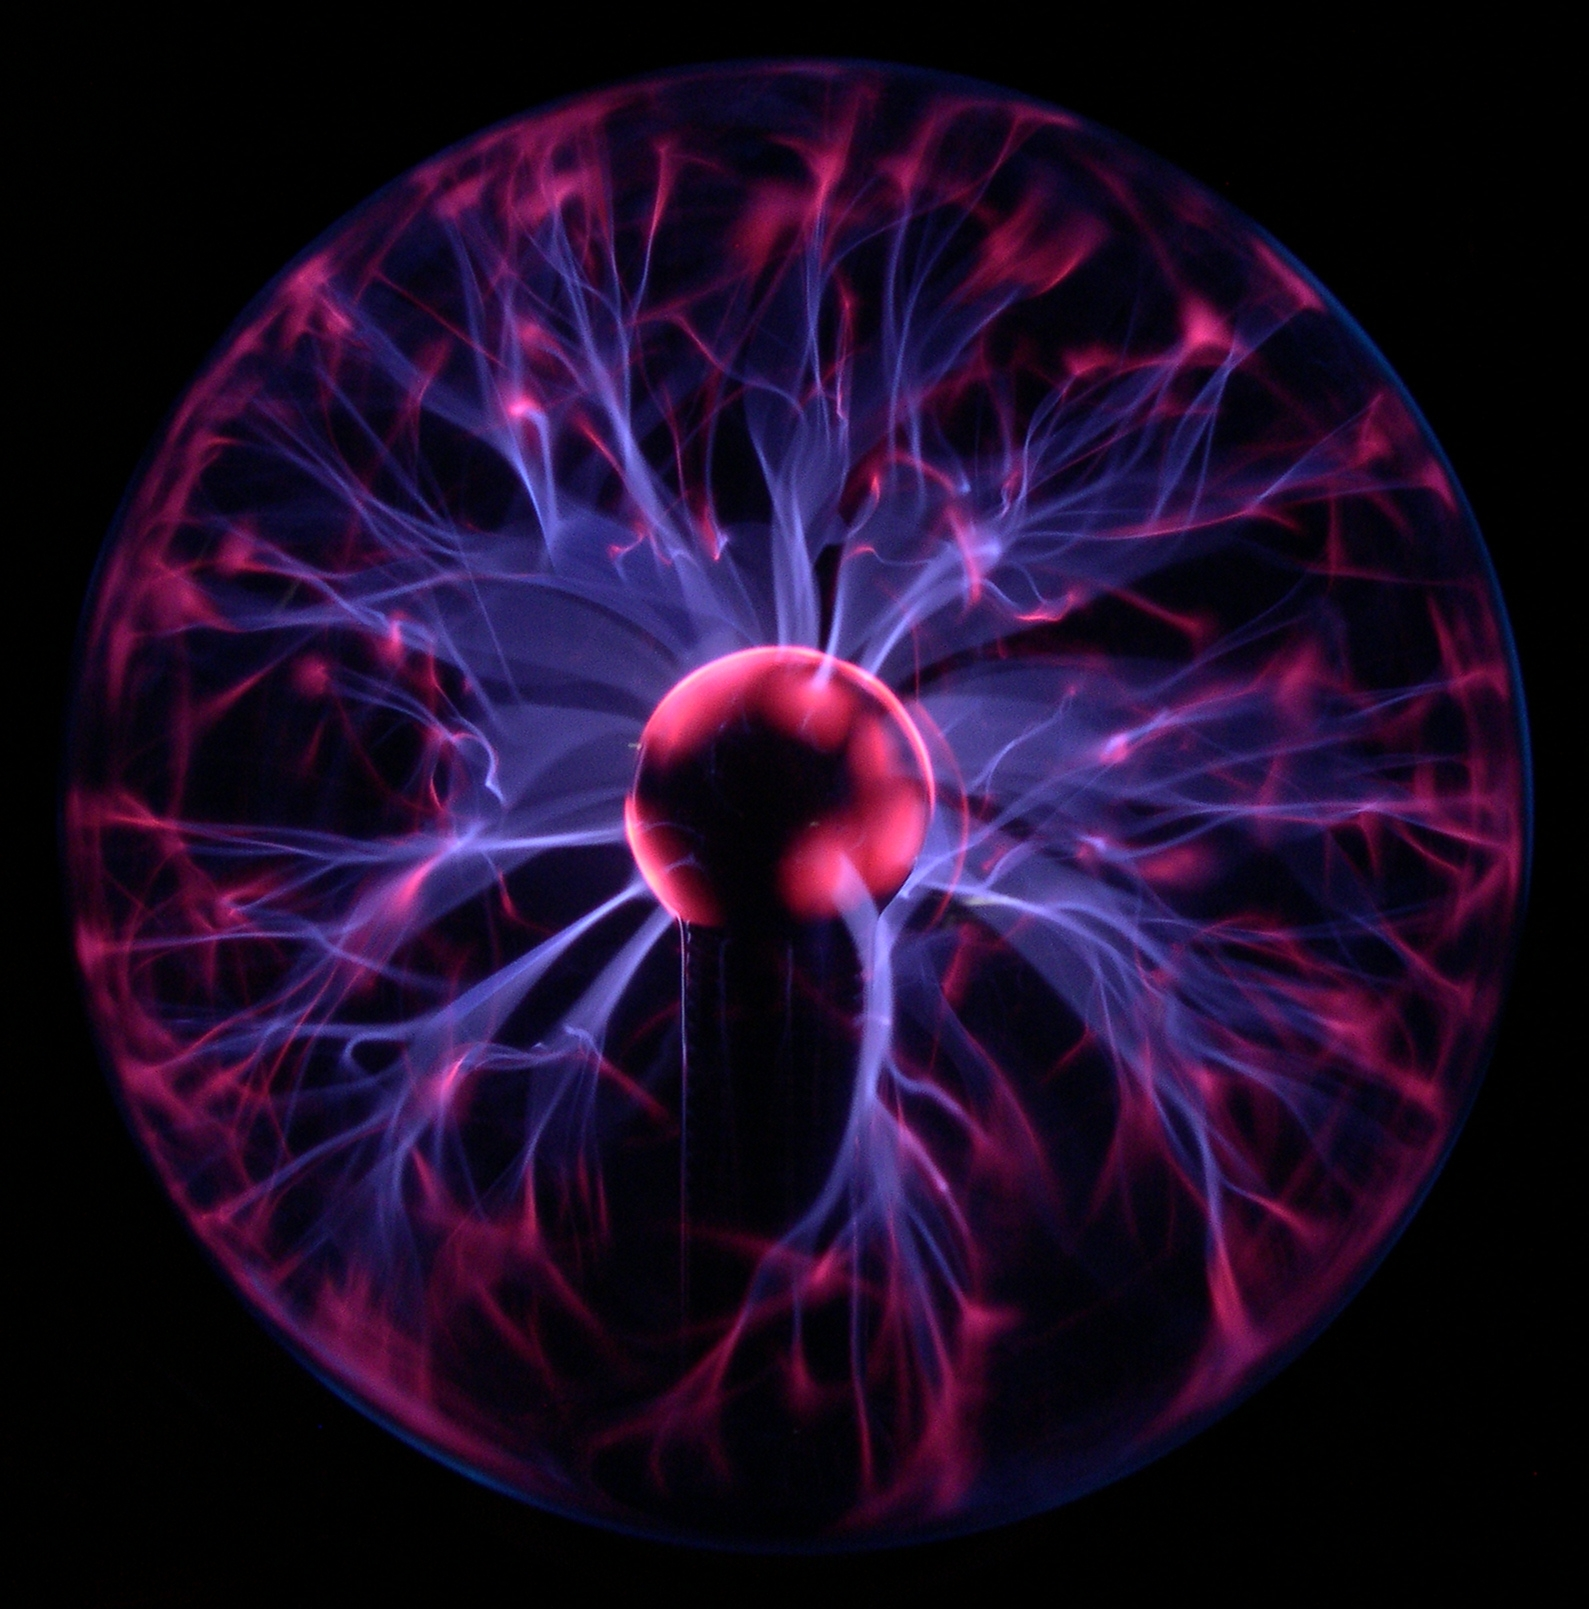
\includegraphics[width=0.55\textwidth, height=3cm]{Lampara_plasma.jpg}
            %\caption{}
            \label{fig:im1}
        \end{figure}

        \begin{figure}
            \centering
            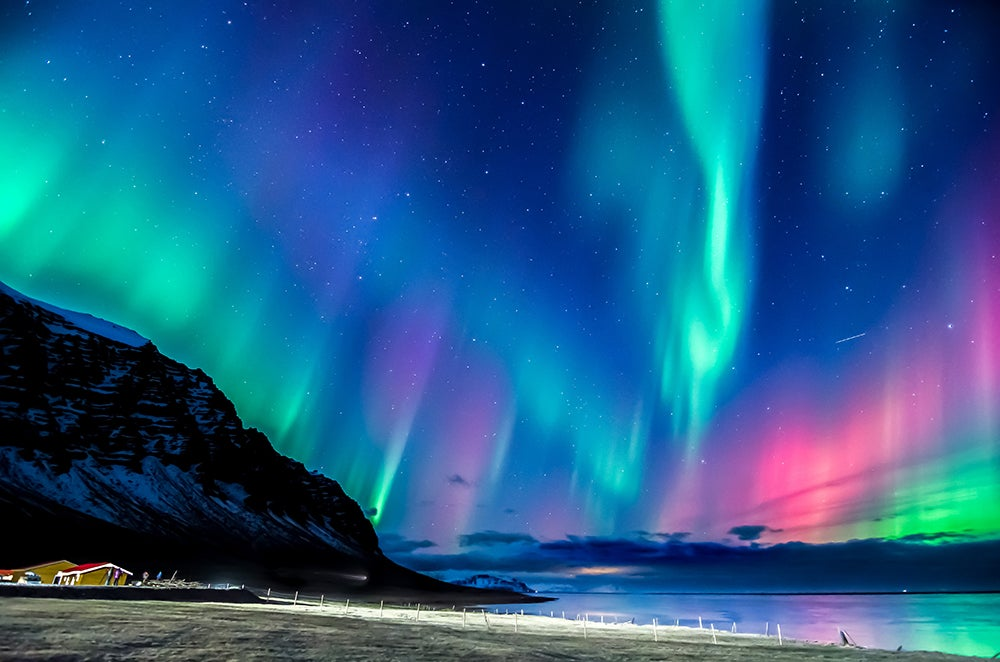
\includegraphics[width=0.8\textwidth, height=2.5cm]{auroras_boreales.jpg}
            %\caption{}
            \label{fig:im2}
        \end{figure}
        \end{column}
        \end{columns}
        
        \end{frame}
        
        \begin{frame}[t]{¿Qu\'e es un plasma?}
        %\vspace{1em}
        \begin{itemize}
        %\fontsize{14pt}{15}\selectfont
        \fontsize{11pt}{15}\selectfont
        \item<cir@1-> Debido a la complejidad de las interacciones, y la naturaleza de las partículas, dentro del plasma se pueden describir una gran variedad de fenómenos.   \\ 
        Ejemplos: Ondas de Alfvén, radiación sincrotrón, inestabilidades magnetohidrodinámicas, etc. 
        \item<cir@1-> Tecnológicamente, son usados en la modificación de superficies, purificación de materiales, materia prima para futuros procesos de producción de energía limpia (fusión nuclear), etc. 
        \end{itemize}
    
        \begin{figure}
        \centering
        {\subfigure{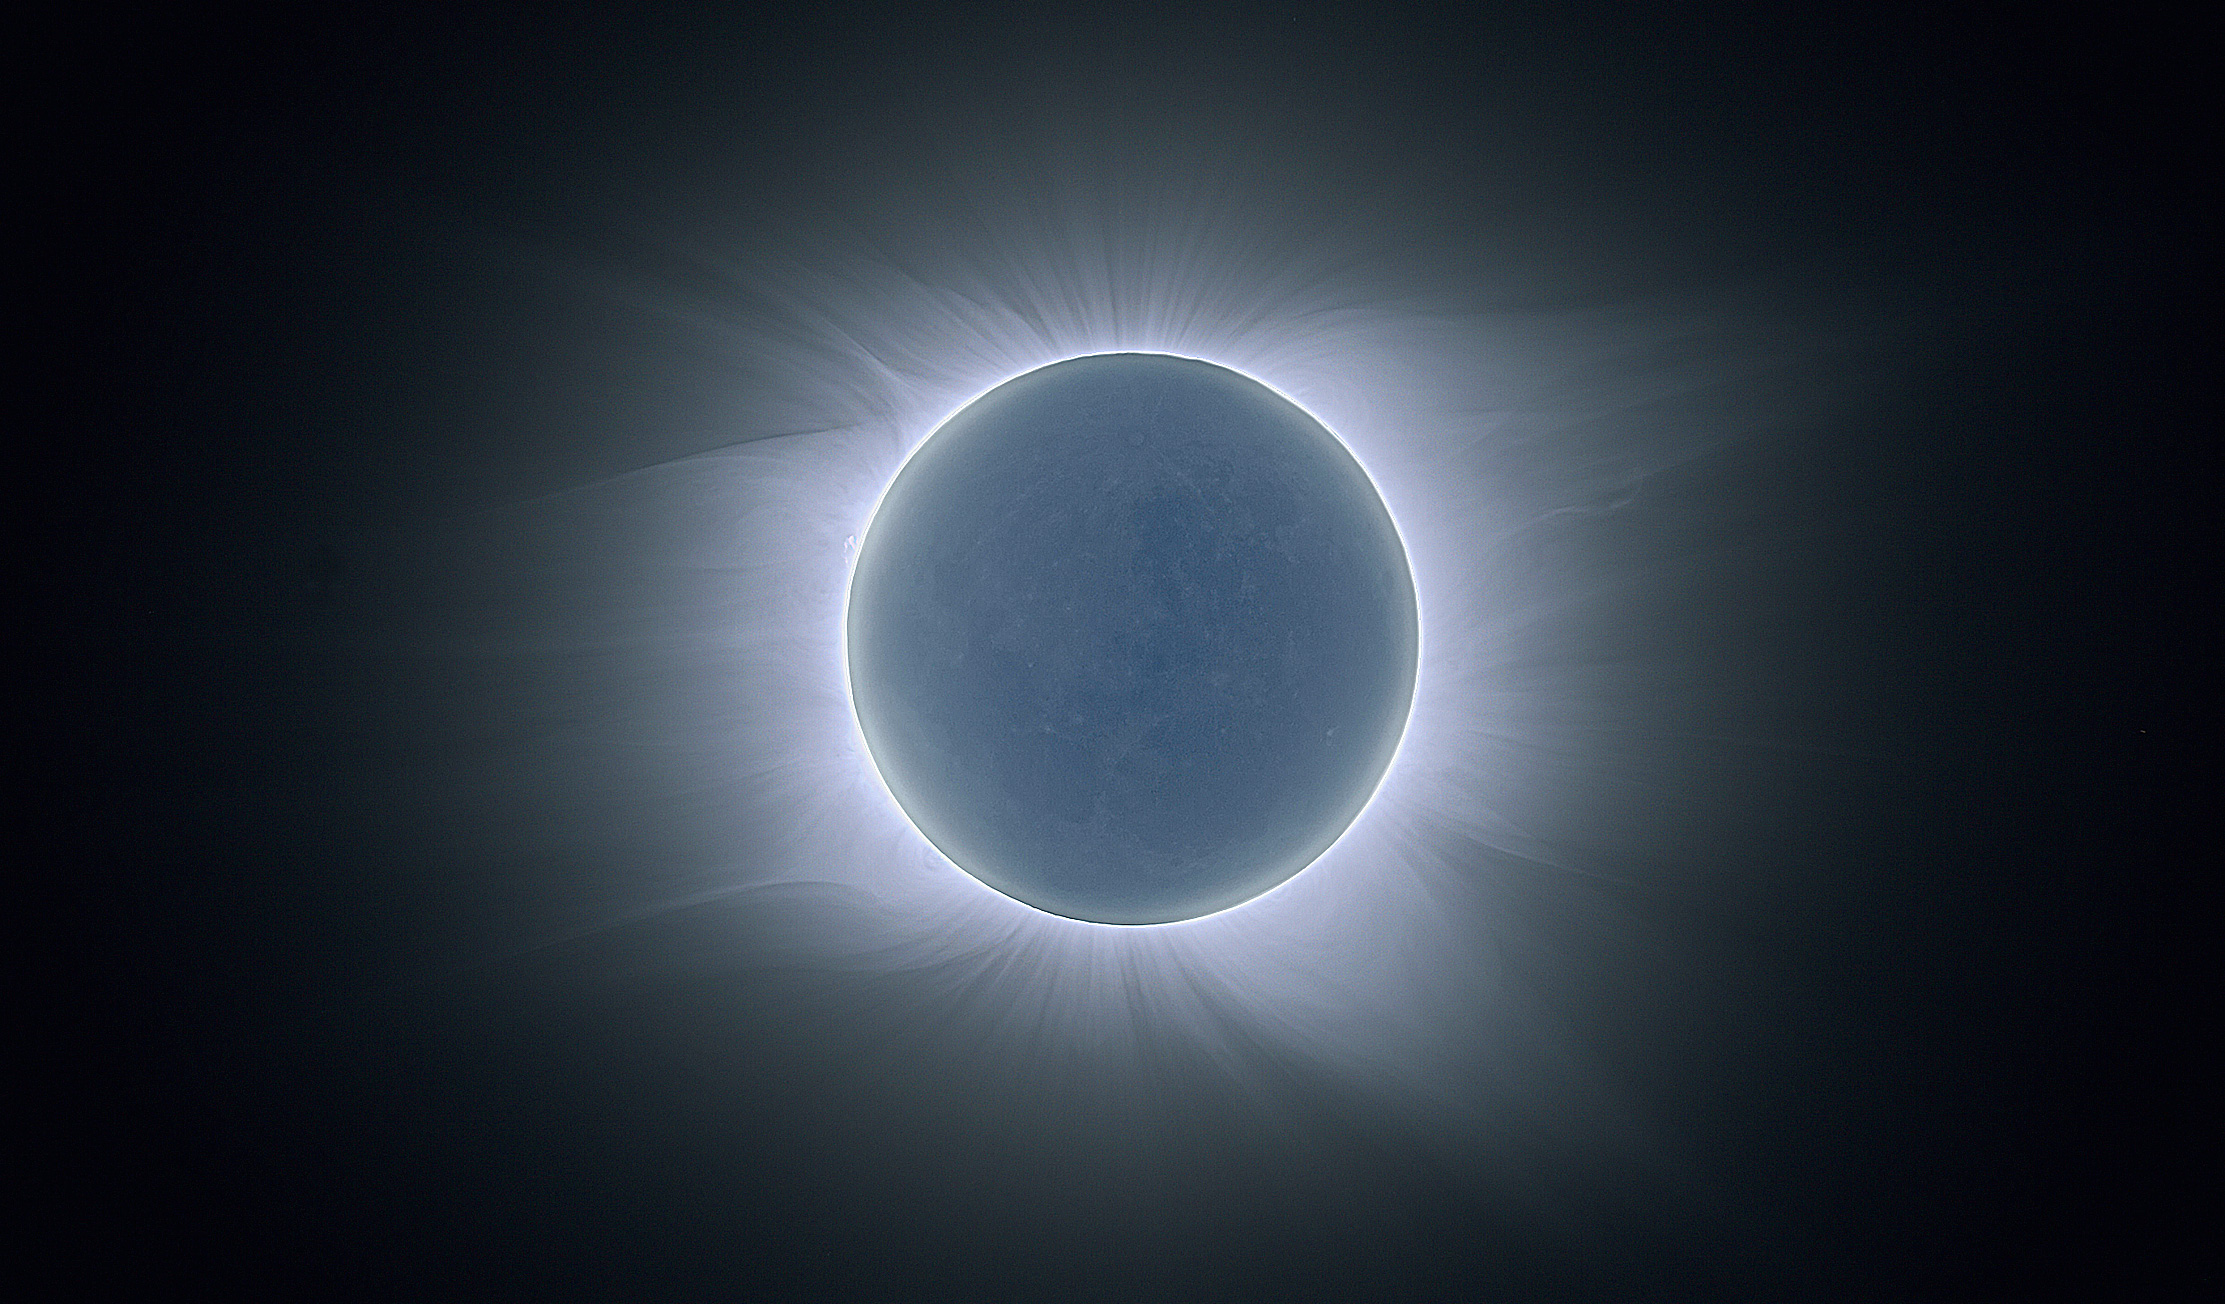
\includegraphics[width=4cm,height=2.2cm\textwidth]{corona_solar.jpeg}}}
        {\subfigure{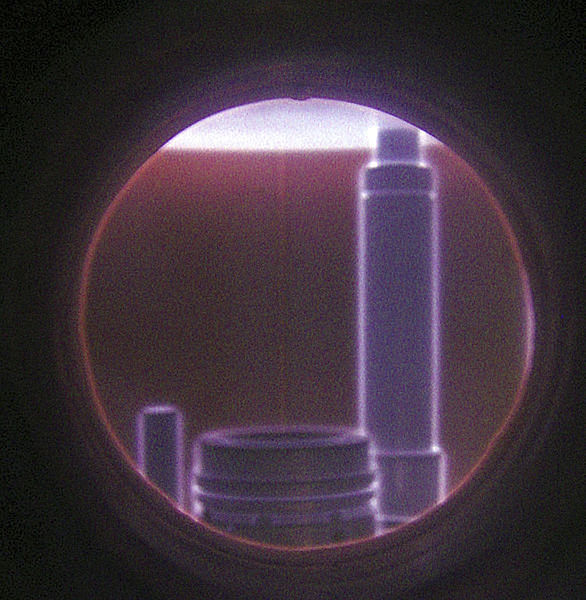
\includegraphics[width=2.2cm,height=2.2cm]{purificacion_materiales.jpg}}} 
        \end{figure}
    
        \end{frame}
        

    \section{Propiedades b\'asicas}
        
       

    \subsection{Apantallamiento y longitud de Debye}
        \begin{frame}{Apantallamiento y longitud de Debye}
        
        \fontsize{8pt}{10}\selectfont
        %\vspace{} % Para agregar espacio despues del título del frame y el bloque
        \begin{columns}
        \begin{column}{0.4\textwidth}
        \begin{block}{}
            \begin{itemize}
            \item Potencial el\'ectrico de una partícula cargada aislada:
            \begin{align*}
                \phi = \frac{q}{4\pi\epsilon_0r}
            \end{align*}
            \item Potencial el\'ectrico de una partícula inmersa en el plasma: 
            \begin{align*}
                \phi_D = \phi e^{\frac{-r}{\lambda_D}}.
            \end{align*}
            \item Cualquier potencial dentro de un plasma es apantallado, más allá de cierta distancia (longitud de Debye):
            \begin{align*}
            \lambda_D = \left(\frac{k_BT\epsilon_0}{e^2n}\right)^{1/2}.
        \end{align*}
        \end{itemize}
        \end{block}
        \end{column}
        
        \begin{column}{0.5\textwidth}
        \begin{figure}
            \centering
            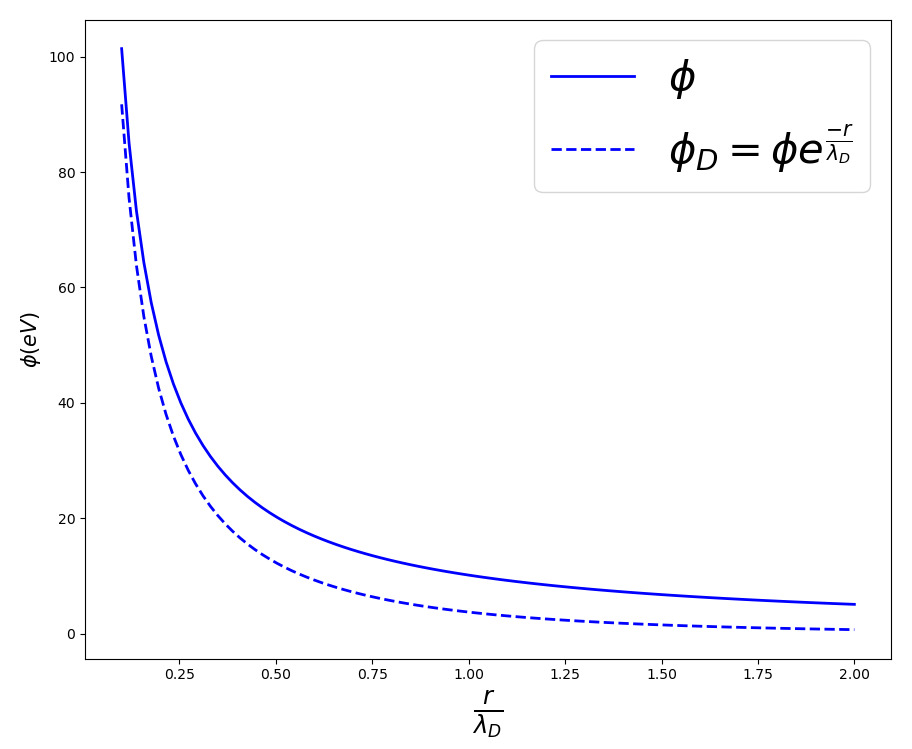
\includegraphics[width=\textwidth]{Potencial_modificado.jpg}
            \caption{Potencial de Debye $\phi_D$}
            \label{fig:imag1}
        \end{figure}
        \end{column}
        \end{columns}
        
        \end{frame}
        
    \subsection{Frecuencia del plasma}
        \begin{frame}{Frecuencia del plasma}
        \fontsize{8pt}{10}\selectfont        \begin{columns}
        \begin{column}{0.4\textwidth}
        \begin{block}{}        
        \begin{itemize}
        \item Los desplazamientos en la densidad de carga en el plasma producen campos eléctricos:
        \begin{align*}
        &n_e(x,t) = n_0 + \tilde{n}_e(x,t),\\
        &\vec E(x,t) = \vec E_0 + \tilde{\vec E}(x,t).
        \end{align*}
        \item Se producen oscilaciones por parte de las partículas cargadas:
        \begin{align*}
        \frac{\partial^2 \tilde{n}_e(\vec{r},t)}{\partial t^2} + \omega_e^{2} \tilde{n}_e(\vec{r},t) = 0.
        \end{align*}
        \item Se tiene que la frecuencia del plasma es:
        \begin{align*}
        \omega_e = \left( \frac{e^2n_0}{m_e\epsilon_0} \right)^{1/2}.
        \end{align*}
        \end{itemize}
        \end{block}
        \end{column}
        
        \begin{column}{0.4\textwidth}
        \begin{figure}
            \centering
            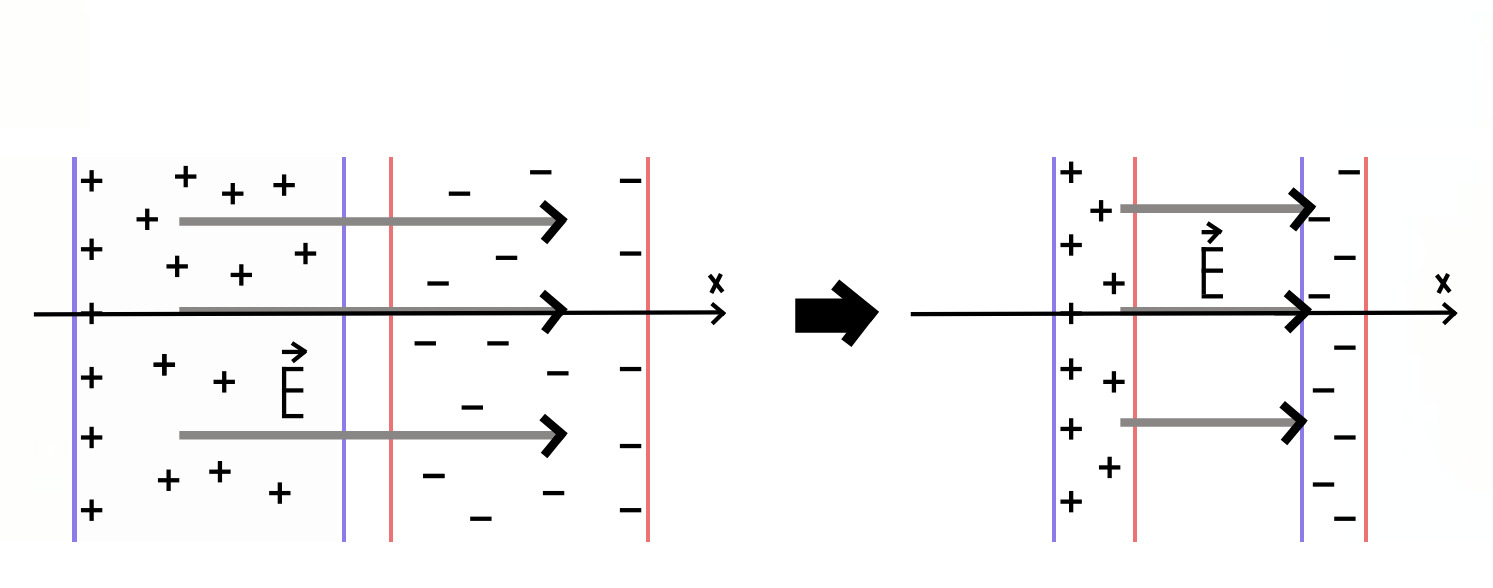
\includegraphics[width=5cm,height=3cm]{frecuencia_plasmas.jpg}
            \caption{Desplazamiento de cargas}
            \label{fig:imag2}
        \end{figure}
        \end{column}
        \end{columns}
        
        \end{frame}
        
    \subsection{Par\'ametro del plasma}
        \begin{frame}{Par\'ametro del plasma}
        \fontsize{7pt}{9}\selectfont
        \begin{columns}
        \begin{column}{0.4\textwidth}
        \begin{block}{}        
        \begin{itemize}
            \item Se calcula una distancia de máximo acercamiento, y se define una distancia media entre partículas respectivamente:
            \begin{align*}
            &d_a = q/4\pi\epsilon_0k_BT,\\
            &d_m \equiv 1/n^{1/3}.
            \end{align*}
            \item Se define el par\'ametro del plasma como:
            \begin{align*}
             \Lambda = 4\pi n\lambda^3_D = \frac{1}{\sqrt{4\pi}}\left(\frac{d_m}{d_a}\right)^{3/2}.
            \end{align*}
            \item Plasmas fuertemente acoplados
            \begin{align*}
            d_m \ll d_a \rightarrow \Lambda \ll 1
            \end{align*}
            \item Plasmas debilmente acoplados
            \begin{align*}
                d_a \ll d_m \rightarrow \Lambda \gg 1
            \end{align*}
        \end{itemize}
        \end{block}
        \end{column}
        
        \begin{column}{0.4\textwidth}
        \begin{figure}
            \centering
            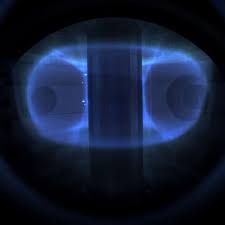
\includegraphics[width=\textwidth, height=3.5cm]{parametro_plasma.jpeg}
            \caption{Plasma debilmente acoplado}
            \label{fig:my_label}
        \end{figure}
        \end{column}
        \end{columns}
        
        \end{frame}

    \section{Fusión nuclear y reactores de fusión}
        \begin{frame}{Fusión nuclear y reactores de fusión}
        \fontsize{8pt}{10}\selectfont
        \begin{columns}
        \begin{column}{0.4\textwidth}
        \begin{block}{}
        \begin{itemize}
            \item La fusión nuclear consiste en acercar los núcleos de dos átomos ligeros, para que puedan reaccionar y convertir masa en energía. 
            \item Al acercarse lo suficiente, la fuerza nuclear fuerte predomina sobre la fuerza electrostática. 
            \item Las partículas generadas llevan la energía producida en forma de energía cinética. 
            \item Para una reacción de deuterio-tritio: 
            \fontsize{7pt}{9}\selectfont
            \begin{align*} \mathrm{\tensor^2{H}{}+\tensor^3{H}{} &\longrightarrow  \mathrm{\tensor^4{He}{}+\tensor^1{n}{}}}, \\ \vspace{2em}
            E = 2.818\times&10^{-12} \ \mathrm{J} = 17.59 \ \mathrm{MeV}.
            \end{align*}
    
        \end{itemize}
        \end{block}
        \end{column}
        
        \begin{column}{0.4\textwidth}
        \begin{figure}
        \centering
         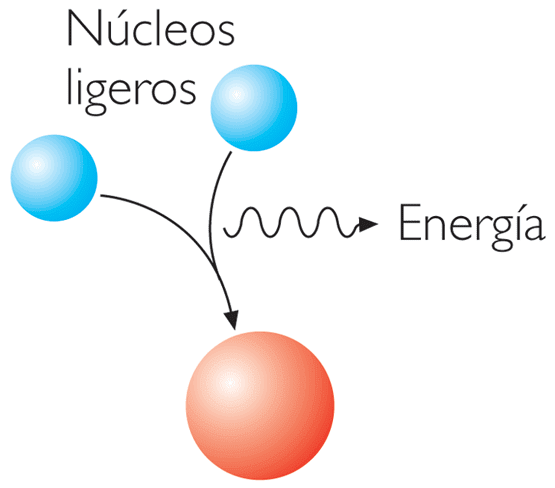
\includegraphics[width=0.8\textwidth]{fusion_nuclear1.png}
        \caption{En el proceso, se fusionan dos núcleos ligeros para formar uno más pesado.}
        \label{fig:fusion}
        \end{figure}
        \end{column}
        
        \end{columns}
        \end{frame}

        \begin{frame}[t]{Fusión nuclear y reactores de fusión}
        \fontsize{9pt}{11}\selectfont
       
        \begin{block}{}
        \begin{itemize}
            \item Contenedores de plasma a altas temperaturas.
            \item Tokamak: reactor de fusión en forma de donut.
            \item Campos magnéticos toroidales y poloidales. Se producen superficies de flujo magnético.
            \item Balance entre la potencia suministrada, perdida, y producida en el plasma. Criterio de Lawson.     
        \end{itemize}
        \end{block}
        
        \begin{figure}
        \centering
         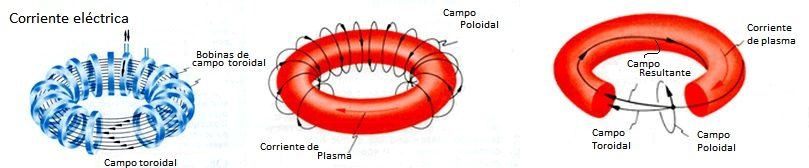
\includegraphics[width=0.9\textwidth,height=3cm]{campos_magn.jpg}
        %\caption{En el proceso, se fusionan dos núcleos ligeros para formar uno más pesado.}
        \label{fig:fusion}
        \end{figure}
       

        \end{frame}


    \section{Scrape Off Layer (SOL)}
        \begin{frame}{Scrape Off Layer (SOL)}
        
        \fontsize{7pt}{9}\selectfont
        \begin{columns}
        \begin{column}{0.4\textwidth}
        \begin{block}{}
        \begin{itemize}
            \item Superficies de flujo magnético abiertas y cerradas. LCFS (Last closed flux surface).
            \item Región externa del plasma denominada Scrape Off Layer (SOL).
            \item Grosor de la SOL:
            \begin{align*}
               L_{SOL} \approx 10^{-2} \ m.
            \end{align*}
            \item Razón entre la velocidad de campo cruzado y paralelo:
            \begin{align*}
            &v_{\perp} \approx 10^2 \ ms^{-1} \\
            &v_{\parallel} \approx c_s \approx 3\times10^5 \ ms^{-1}, \\
         \rightarrow 
         &\frac{v_{\parallel}}{v_{\perp}}\approx 3000
            \end{align*}
        \end{itemize}
        \end{block}
        \end{column}
        
        \begin{column}{0.4\textwidth}
        \begin{figure}
        \centering
         \includegraphics[width=0.9\textwidth]{SOL_LCFS.jpg}
        \caption{Vista tranversal de un reactor Tokamak.}
        \label{fig:sol}
        \end{figure}
        \end{column}
        
        \end{columns}
            
        \end{frame}
        
    \section{Condición de Bohm}
    
    \subsection{Ti=0}
        \begin{frame}{Condici\'on de Bohm: Ti = 0}
            \fontsize{8pt}{10}\selectfont
        
        \begin{itemize}
            \item Se estudia la dinámica del plasma externo o de borde (SOL) y su interacción con las superficies materiales. 
            \item Para un plasma a altas temperaturas, se puede usar con buena aproximación, una distribución de velocidades de Maxwell:
            \begin{align*}
	        f_{\alpha}\left(\mathbf{v}_{\alpha}\right) = n_{\alpha}\left(\frac{m_{\alpha}}{2\pi k_BT_{\alpha}}\right)^{3/2}exp\left(-\frac{m_{\alpha}v_{\alpha}^2}{2k_BT_{\alpha}}\right).
	        \end{align*}
            \item Para dos especies contenidas en el plasma (iones y electrones) se tiene que la razón en el flujo aleatorio es:
             \begin{align*}
            &\Phi_{\alpha} = \frac{1}{4}n_{\alpha}<v>_{\alpha} \ \rightarrow  \ \Phi_{\alpha} = n_{\alpha} \left( \frac{kT_{\alpha}}{2\pi m_{\alpha}} \right)^{1/2} \ \rightarrow \ \frac{\Phi_{e}}{\Phi_{i}} \approx 85.39.
            \end{align*}
            \item Debido a que se tiene un mayor flujo de electrones, cerca a una superficie material, estos tenderán a acumularse más rápido. Aparecerá un potencial de pared.
        \end{itemize}
        \end{frame}
        
        \begin{frame}[t]{Condici\'on de Bohm: Ti = 0}
        \fontsize{7pt}{9}\selectfont
        \begin{columns}[t]
        \begin{column}{0.4\textwidth}
        \begin{itemize}
            \item Potencial limitado por el apantallamiento. Región de desbalance de cargas.
            \item Modelo unidimensional.
            \item Temperatura iónica igual a cero.
            \item \'Unica fuente de iones.
            \item Sin colisiones.
        \end{itemize}
        \begin{figure}
        \centering
        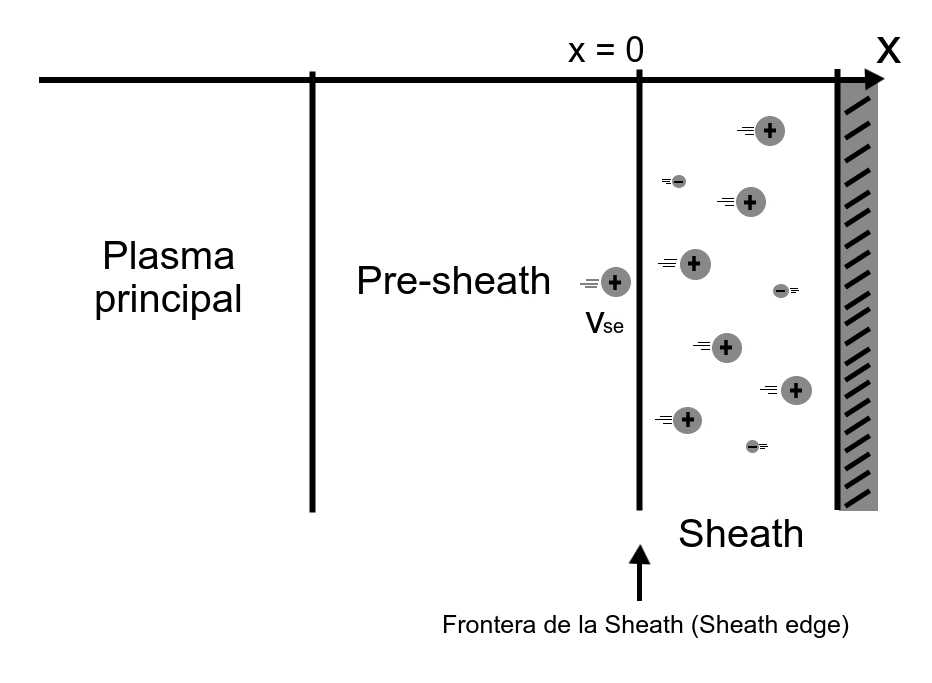
\includegraphics[width=0.9\textwidth]{sheath_edge.jpg}
        %\caption{Caption}
        \label{fig:regiones}
        \end{figure}
        \end{column}
        
        \begin{column}{0.5\textwidth}
        \fontsize{6pt}{8}\selectfont
        Por la conservación de energía, y flujo de partículas
        \begin{align*}
        &\frac{1}{2} m_i v_i^2(x) = \frac{1}{2} m_i v_{se}^2 - e\phi(x), \\
        &n_i(x)v_i(x) = n_0v_{se}.\\ \\
        \rightarrow \ &n_i(x) = n_0\left(1 - \frac{2e\phi \left(x\right)}{m_i}v_{se}^2\right)^{-1/2}, \\
        \rightarrow \ &n_e\left(x\right) = n_0exp\left(\frac{e\phi\left(x\right)}{k_BT_e}\right).
        \end{align*}
        %\begin{block}{}
        Resolviendo la ecuación de Poisson
        \begin{align*}
        &\epsilon_0 \frac{d^2\phi}{dx^2} =  en_0\left[exp\left( \frac{e\phi\left(x\right)}{kT_e} \right) - \left(1 -\frac{2e\phi\left(x\right)}{m_i}v_{se}^2 \right)^{-1/2} \right], \\
        &\chi \equiv -\frac{e\phi}{k_BT_e}, \ \xi \equiv \frac{x}{\lambda_D}, \ M = \frac{v_{se}}{\left( kT_e/m_i \right)^{1/2}}, \\
        \rightarrow \ &\frac{d^2\chi}{d\xi^2} = \left( 1+\frac{2\chi}{M^2} \right)^{-1/2} - exp\left( -\chi \right).
        \end{align*}
        %\end{block}
        \end{column}
        
        \end{columns}
        \end{frame}

    \begin{frame}{Condici\'on de Bohm: Ti = 0}
        \fontsize{8pt}{10}\selectfont
        
        %\begin{block}{}
        \begin{itemize}
            \item Mediante la aproximación:
            \begin{align*}
              \chi \ll 1,
            \end{align*}
           se tiene
           \begin{align*}
           \frac{1}{2}\chi^2\left(-\frac{1}{M^2}+1\right) &\geq 0,\\
              M^2 &\geq 1, \\
              v_{se} &\geq \left(\frac{k_BT_e}{m_i}\right)^{1/2}
            \end{align*}
            \item Se tiene entonces que la velocidad con la que ingresan los iones a la sheath, es mayor que la velocidad del sonido del plasma:
            \begin{align*}
                v_{se} \geq c_s
            \end{align*}
            \item Velocidad del sonido del plasma a $T_i = 0$:
            \begin{align*}
                c_s = \left(\frac{k_BT_e}{m_i}\right)^{1/2}
            \end{align*} 
        \end{itemize}
        %\end{block}
        
        \end{frame}
        
        \begin{frame}[t]{Condici\'on de Bohm: Ti = 0}
        
        \fontsize{9pt}{11}\selectfont
        \begin{columns}
        \begin{column}{0.4\textwidth}
        \begin{block}{}
        \begin{itemize}
            \item Sheath: Región más cercana a la pared. Desbalance en la densidad total de cargas.
            \vspace{2em}
            \item Presheath: Pequeña caída de potencial. Región de aceleración. Neutralidad.
            \vspace{2em}
            \item Plasma principal: Potencial igual a cero. Neutralidad macrosc\'opica.
        \end{itemize}
        \end{block}
        \end{column}
        
        \begin{column}{0.5\textwidth}
        \begin{figure}
        \centering
         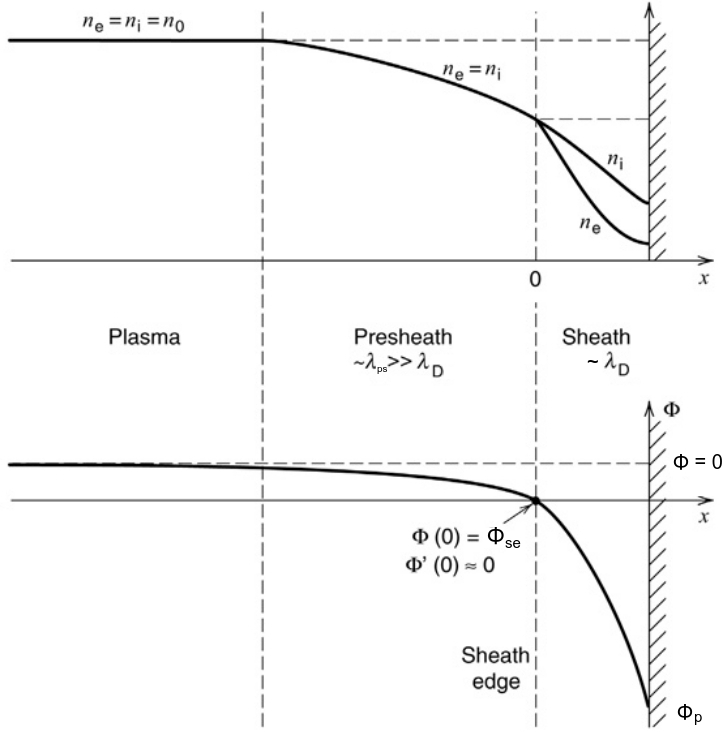
\includegraphics[width=0.9\textwidth,height=6cm]{grafica_bohm_curvas.jpg}
        %\caption{}
        %\label{fig:fusion}
        \end{figure}
        \end{column}
        
        \end{columns}
            
        \end{frame}
    
        \begin{frame}[t]{Condici\'on de Bohm: Ti = 0}
            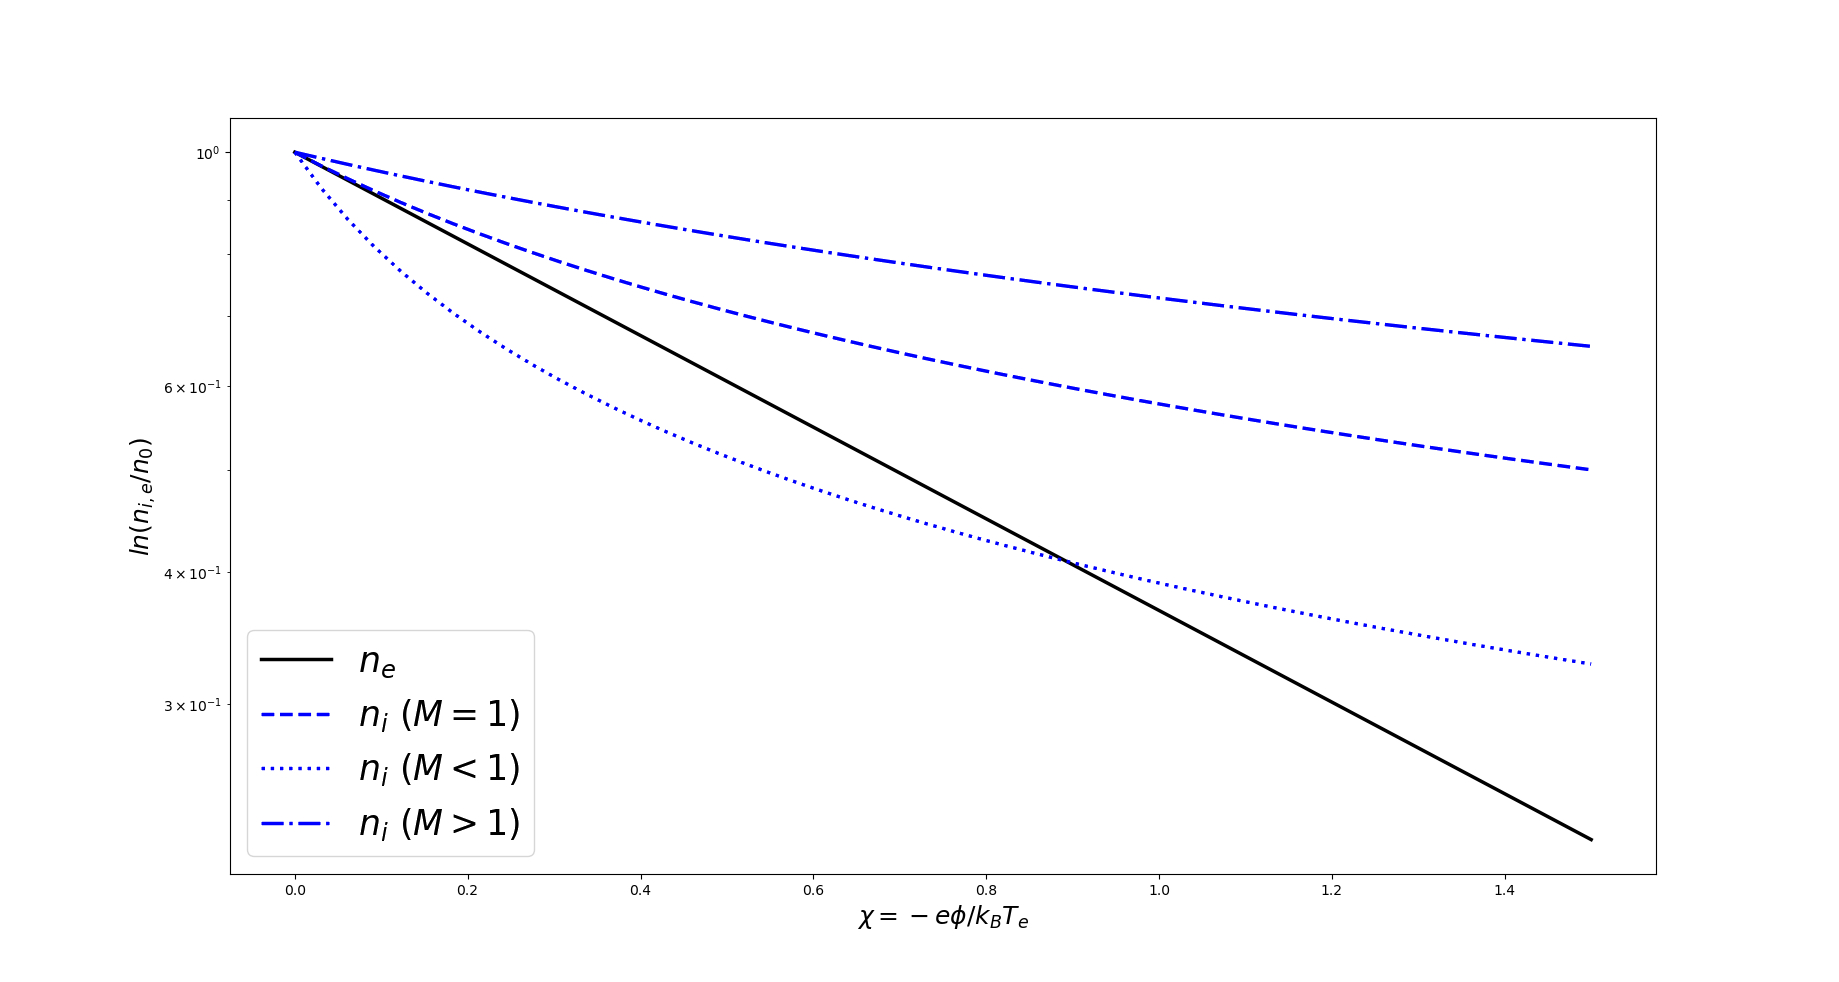
\includegraphics[scale=0.195]{dens4.jpg}
        \end{frame}
        %\subsection{$Ti = 0$}
        %\begin{frame}{$Ti=0$}
            
        %\end{frame}
        
        %\subsection{$Ti \neq 0$}
        %\begin{frame}{$T_i \neq 0$}
            
        %\end{frame}
    \subsection{Ti \neq 0 }
        \begin{frame}{Condici\'on de Bohm: Ti \neq 0}
        \fontsize{7pt}{9}\selectfont
        
        %\begin{block}{}
        \begin{itemize}
            \item Se deduce una condición de frontera para la densidad total de carga:
            \begin{align*}
                \frac{d\rho}{d\phi} \leq 0\hspace{1em}y\hspace{1em}\rho = \sum_p q_pn_p\hspace{1em} \rightarrow\hspace{1em} \sum_p q_p \frac{dn_p}{dx} \geq 0.
            \end{align*} 
            \item Calculando la densidad total mediante las distribuciones de velocidades:
            \begin{align*}
                n_p = \int_{-\infty}^{\infty} f_p dv_x \ \rightarrow \
                \sum_p q_p \int_{-\infty}^{\infty}\frac{\partial f_p}{\partial x}dv_x \geq 0.
            \end{align*} 
            \item Ecuación de Boltzman. Eliminando la parte temporal y el término de colision se obtiene la ecuación de Vlasov:
            \begin{align*}
                \frac{\partial f_p}{\partial t} + \vec v\cdot\frac{\partial f_p}{\partial \vec r} +\frac{\vec F}{m_p} \cdot\frac{\partial f_p}{\partial \vec v} = C\left(f_p\right)\hspace{1em}\rightarrow\hspace{1em}
                 v_x\frac{\partial f_p}{\partial x} + \frac{q_p}{m_p}E\frac{\partial f_p}{\partial v_x} = 0.
            \end{align*} 
            \begin{align*}
                 \frac{1}{m_i} \int_{-\infty}^{\infty} \frac{1}{v_x}\frac{\partial f_i}{\partial v_x}dv_x \leq  -\frac{1}{m_e} \int_{-\infty}^{\infty} \frac{1}{v_x}\frac{\partial f_e}{\partial v_x} dv_x.
            \end{align*}
            
        \end{itemize}
        
        %\end{block}

            
        \end{frame}
   
        \begin{frame}{Condici\'on de Bohm: Ti \neq 0}
        \fontsize{7pt}{9}\selectfont
        %\begin{block}{}
        \begin{itemize}
            \item Condición generalizada de Bohm:
            \begin{align*}
                 \frac{1}{m_i} \int_{-\infty}^{\infty} \frac{1}{v_x}\frac{\partial f_i}{\partial v_x}dv_x \leq  -\frac{1}{m_e} \int_{-\infty}^{\infty} \frac{1}{v_x}\frac{\partial f_e}{\partial v_x} dv_x
            \end{align*} 
            \item Mediante una integración por partes (limitada), se tiene: 
            \begin{align*}
                &\int _{-\infty}^{\infty} \frac{1}{v_x}\frac{\partial f_i}{\partial v_x}dv_x = \int_{-\infty}^{\infty}\frac{\partial }{\partial v_x} \left( \frac{f_i}{v_x} \right)dv_x + \int_{-\infty}^{\infty}\frac{f_i}{v_x^2}dv_x, \\ \\ 
                 &\rightarrow \ \frac{1}{m_i} \int_{-\infty}^{\infty} \frac{f_i}{v_x^2}dv_x \leq  -\frac{1}{m_e} \int_{-\infty}^{\infty} \frac{1}{v_x}\frac{\partial f_e}{\partial v_x} dv_x.
            \end{align*} 
            
        \end{itemize}
        %\end{block}
        \end{frame}
   
   \begin{frame}[t]{Condici\'on de Bohm}
    \fontsize{6pt}{8}\selectfont
   \begin{columns}
   \begin{column}{0.4\textwidth}
   \begin{figure}
       \centering
       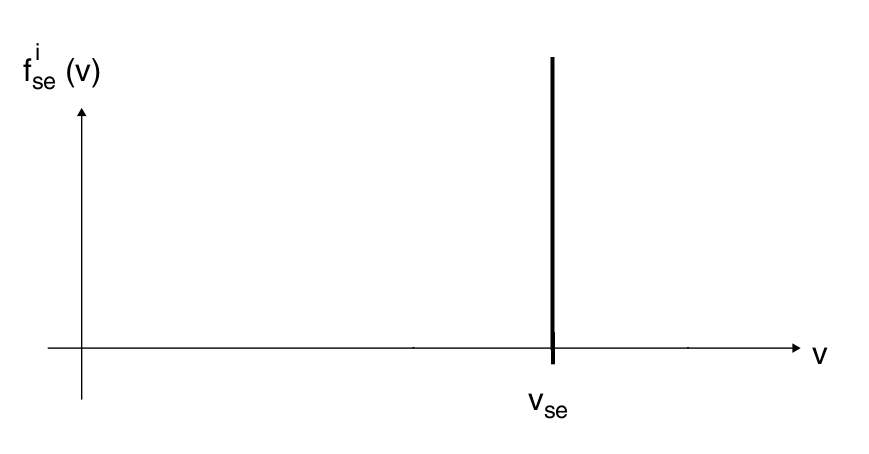
\includegraphics[width=\textwidth]{delta.jpg}
       \caption{Distribuci\'on de velocidades para $Ti=0$ (Funci\'on delta de Dirac)}
       \label{fig:my_label}
   \end{figure}
   \begin{align*}
        f_i(v) &= n_0\delta\left(v - v_{se} \right) \\ \\
        \rightarrow \ v_{se} &\geq \left(\frac{k_BT_e}{mi}\right)^{1/2}
    \end{align*} 
   \end{column}
   
   \begin{column}{0.4\textwidth}
   \begin{figure}
       \centering
       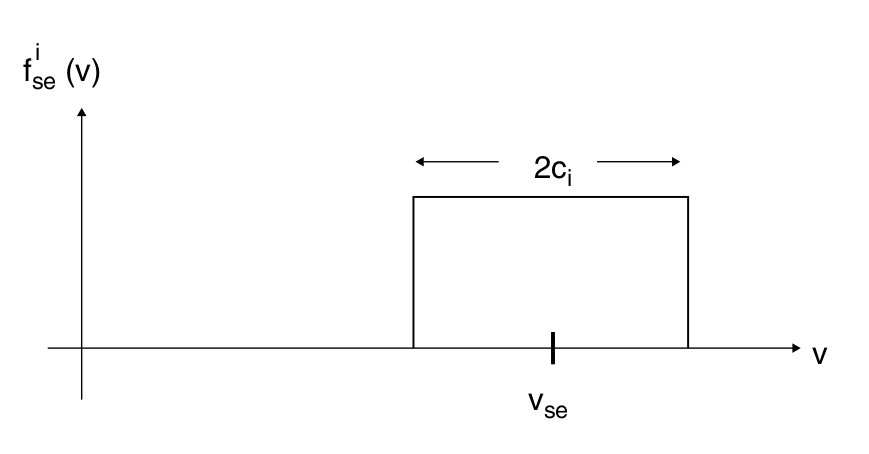
\includegraphics[width=\textwidth]{square.png}
       \caption{Distribuci\'on de velocidades para $Ti\neq0$ (Funci\'on  ``top jat")}
       \label{fig:my_label}
   \end{figure}
   \begin{align*}
        f_i\left(v_x\right) &= \left\{ \begin{array}{lcc}
             n_0\left(2c_i\right)^{-1} & si \ v_{se}-c_i \leq v_x \leq v_{se}+c_i \\
             \\ 0 &  para \ otros \ valores \ de \ v_x
             \end{array}
   \right. \\
   \rightarrow \ v_{se} &\geq \left(\frac{k_BT_e}{m_i} + \frac{k_BT_i}{m_i}\right)^{1/2}
        \end{align*}
   \end{column}
   \end{columns}
   \end{frame}
   
   \section{Conclusiones}
        \begin{frame}{Conclusiones}
            \begin{itemize}
                \item En un plasma, en contacto con alguna superficie, los iones se aceleran hasta ella a través de un potencial eléctrico, hasta alcanzar la velocidad del sonido del plasma. 
                \item Este potencial se produce en las superficies de contacto, por lo que es apantallado debido a las propiedades del plasma. 
                \item Cerca a las superficies de contacto, se genera una región de desbalance en la densidad de carga total.
            \end{itemize}
        \end{frame}

%%%%%%%%%%%%%% Diapositivas %%%%%%%%%%%%%%%

%%%%%%%%%%%%%%%%%%%% Fin %%%%%%%%%%%%%%%%%%%%
\end{document}



 \begin{frame}[t]{Propiedades b\'asicas}
        \fontsize{7pt}{9}\selectfont
        %\vspace{} % Para agregar espacio despues del título del frame y el bloque
        \begin{columns}
        \begin{column}{0.4\textwidth}
        \begin{block}{Title}
        \justify
        El correcto comportamiento del plasma dentro de un reactor, para los fines perseguidos, es objeto de gran estudio e investigación. Una de parte de ello, se encarga de la interacción plasma-pared. Como ya se mencionó, un reactor utiliza potentes campos magnéticos para confinar el movimiento de las partículas cargadas.
        \end{block}
        \end{column}
        
        \begin{column}{0.4\textwidth}
        \begin{block}{Title}
        \justify
        El correcto comportamiento del plasma dentro de un reactor, para los fines perseguidos, es objeto de gran estudio e investigación. Una de parte de ello, se encarga de la interacción plasma-pared. Como ya se mencionó, un reactor utiliza potentes campos magnéticos para confinar el movimiento de las partículas cargadas.
        \end{block}
        \end{column}
        \end{columns}
        
        \end{frame}
